\documentclass[a4paper,12pt,oneside,headsepline]{scrreprt}
%\documentclass[a4paper,12pt,oneside,headsepline]{scrartcl}

\usepackage{ifxetex}
\ifxetex
	\usepackage{fontspec}
		\setmainfont{Gentium}
\fi

\usepackage{graphicx}
\usepackage{longtable}
\usepackage{tabularx}
\usepackage{setspace}
\usepackage{hyperref}
\usepackage{float}
\usepackage{flafter}
\usepackage{xcolor}
\usepackage{titlesec}
\usepackage{fancyhdr}

\pagestyle{fancy}


\hypersetup{%
    pdfborder = {0 0 0}
}

\addtokomafont{chapter}{\color[RGB]{83,88,85}}
\addtokomafont{section}{\color[RGB]{97,105,100}}

\KOMAoptions{parskip=half}
\KOMAoptions{DIV=12}

\onehalfspacing

\suppressfloats[t]
\suppressfloats[b]

%\clearscrheadfoot

%\ihead{Structured and Modular Design -> should be: current chapter}
%\ohead{Page \thepage\  of XXX}
\lhead{\nouppercase{\rightmark} (\nouppercase{\leftmark})}
\chead{}
\rhead{}

\renewcommand{\headrulewidth}{0.4pt}
\renewcommand{\footrulewidth}{0.4pt}

\renewcommand{\sectionmark}[1]{\markright{\MakeUppercase{#1}}{}}


\lfoot{Version 1.0}
\cfoot{\bfseries \thepage}
\rfoot{\today}

\fancypagestyle{plain}{%
\fancyhf{} % clear all header and footer fields
\fancyfoot[C]{\bfseries \thepage} % except the center
\fancyfoot[L]{Version 1.0}
\fancyfoot[R]{\today}
\fancyhead[LO,RE]{\slshape  \leftmark} %
\renewcommand{\headrulewidth}{0.4pt}
\renewcommand{\footrulewidth}{0.4pt}}

\subject{Software Engineering / Book Express}
\title{Structured and Modular Design}

\author{Christoph Wurm, Stefan Lenzen, Christian Hoff}
\date{\today}


\begin{document}
\pagenumbering{roman}
\maketitle
\newpage
\tableofcontents
\newpage
\listoftables
\newpage

\pagenumbering{arabic}
\setcounter{page}{4}

\chapter{Document history}
\begin{longtable}[c]{|p{0.20\textwidth}|p{0.22\textwidth}|p{0.35\textwidth}|p{0.1\textwidth}|}
\hline
Editor(s) & Date & Purpose of editing & Version\\
\hline
\hline
Christian Hoff & March 25th 2011 & First draft & 0.1 \\
All & March 26th 2011 & Completed modular design & 0.2 \\
Stefan Lenzen & March 29th 2011 & Added additional graphics & 0.3 \\
Christoph Wurm & March 29th 2011 & Completed section on function modules & 0.4 \\
All & March 30th 2011 & Final version & 1.0 \\
\hline
\caption{Document history}
\end{longtable}
\newpage
\chapter{Introduction}
The software architecture of a system is the set of structures needed to reason about the system, which comprise software elements, relations among them, and properties of both\footnote{\href{en.wikipedia.org/wiki/Software_architecture}{en.wikipedia.org/wiki/Software\_architecture}}.

All these elements shall be described in the following chapters. The method of \emph{Structured and Modular Design} will be used to describe the architecture of the program core. The operating system environment, including interfaces to existing software, will also be discussed.

The design specification is threefold: In the beginning, a high-level overview over the application design is provided and interfaces to existing programs are described.

Secondly, we will elaborate on the defined function modules. We will conclude with a description of the data modules. Thereby a \emph{Data Dictionary} will be used to outline the format of all stored application data.
\newpage
\chapter{Architectural overview}
As defined in the Software Requirement Specification by Team 2, a web interface will be provided for the customers of BookExpress. This includes both publishers and book stores. Publishers can use this interface to maintain a list of available book titles. For bookstores, the web interfaces provides a convenient way to order books and track the status of pending deliveries.

The web interface will be programmed using \emph{Java Enterprise Edition 6}.

A desktop application will be used by the employees of BookExpress. Compared to the web interface, it provides advanced functionality including the following:
\begin{itemize}
\item View the status of all pending orders
\item Starting the book delivery process
\item View business report and statistics
\end{itemize}

In addition a mobile client application is provided, which is going to be used by the employees working in the warehouse department. This system aims to support the employees during stock-keeping. It will pop up a notification whenever a book has been ordered. The application then shows the location of the ordered book in the warehouse such that the staff can easily find the ordered book. The software application will then ensure that one parcel is created for each bookstore, which contains the ordered books and an invoice.

\chapter{Interfaces to existing software}
The BookExpress software depends on other software products for some auxiliary functionality. The interfaces to these programs will be described in this chapter.
\section{DB2 database interface}
Certain data of the BookExpress software including customer and order information has to be stored in a persistent way. For this purpose, an existing database software will be used.

\emph{DB2} is a relational database software solution by IBM. We have chosen DB2 mainly because it focuses on business customers with high demands concerning performance, availability and support. It is also a mature programm which runs on many different platforms including(but not limited to) Linux, z/OS and Windows.

\emph{Java DataBase Connectivity(JDBC)} is a java binding which provides access to a wide range of relational databases including DB2. JDBC will serve as the binding between the BookExpress software and the database. Being a part of the Java framework, it also runs on every platform that is supported by Java.

\emph{Hibernate} is an object-relation model which maps entities in database tables to their corresponding Java classes. We will use Hibernate to make the database entities accessible in an object-oriented manner.
\section{TomTom navigation interface}
Usually a truck will deliver parcels to many bookstores, which makes a fast and efficient calculation of the delivery route necessary. For this reason, BookExpres relies on \emph{TomTom Navigator 7}, which will the route calculation and serve as a navigation system.

TomTom provides an \emph{Application Programming Interface(API)} which makes the functions of TomTom accessible to other programs. BookExpress will use this API in order to calculate the fastest route to the bookstores. As soon as a truck becomes available, the API enables the route to be trasnferred to this specific truck automatically.
\chapter{Design overview}
The application design has been created using a method in Software Engeneering known as \emph{Structured and Modular Design}. As such, it includes data and function modules which have been arranged in three layers: User Interface layer, business layer and database layer.

A design overview is provided in the picture below. For your convenience, we have included a more detailed illustration of each function module in the following chapter.

\begin{figure}[H]
\centering
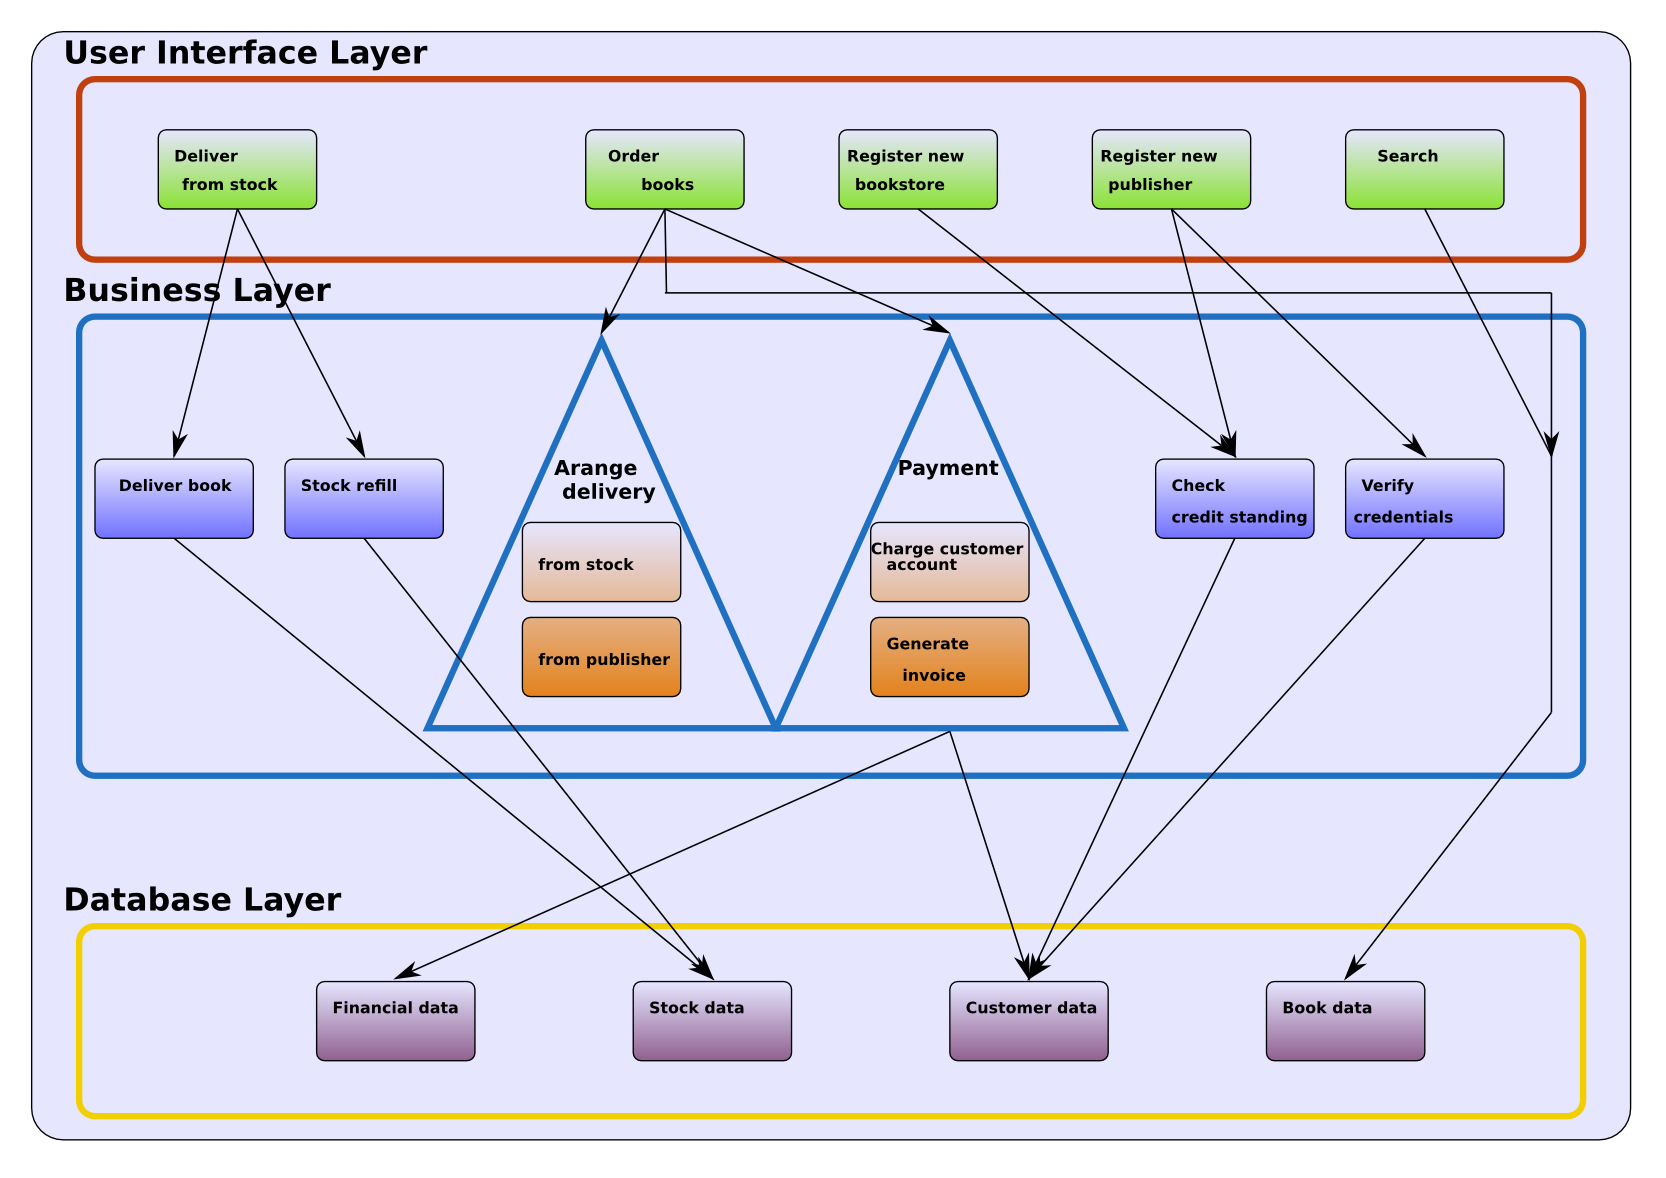
\includegraphics[scale=0.75,angle=270]{Modular_design.png}
\caption{Modular design overview}
\end{figure}

As already mentioned above, the document is divided into three layers. Functionality that should be made visible to the user is located in the top layer - the \emph{User Interface Layer}.

Functions in the User Interface Layer rely on methods in the \emph{Business Layer} for data manipulation. The Business Layer is where the actual business logic is implemented, while the User Interface Layer provides a convenient frontend to the user.
\chapter{Module documentation}
In this section all modules and their connections, dependencies and calling hierarchies will be explained.

\section{\texttt{Order book}}
This is one of the two high-level functions directly called by the user.

When calling this function the bookstore has already determined (perhaps with the help of the function \texttt{Search})
which books it wants to order.

For the function to do its work, the user has to submit the ISBN numbers and quantities of each book he wants to order.
All other information, e.g. whether to deliver from stock or from publisher or where to deliver the order will be automatically
performed by the \emph{BookExpress} system from other data sources (in this case, the stock and customer databases).

When called, the function \texttt{Order book} has to perform several steps:
\begin{enumerate}
	\item Validate user-supplied data.

		  \begin{description}
		  	\item[ISBN numbers] Check if these are valid by looking them up in \emph{BookExpress'} extensive book database.
			\item[Quantities]   Perform a plausibility check. If a small-town bookstore is suddenly ordering five-digit amounts of books,
			                    there is probably something wrong.

								It will still be possible to place such an order, but only after it has been verified, e.g. by phone.
			\item[User credentials] Username and password have to be valid, of course.
		  \end{description}
   \item The order, which we can now be sure of being valid and coming from one of the customers, is entered into the database.
   \item Two things have to be done for the order to be successfully completed: Payment and delivery. Thus, control flow is passed to the
         two modules \texttt{Payment} and \texttt{Arrange delivery}.
\end{enumerate}

\section{\texttt{Payment}}
Every order has to be paid for.

Every customer has a virtual monetary account in the \emph{BookExpress} system that is charged for each order. Simultaneously, an invoice
is generated.

At the end of each month, the virtual account's balance is collected from the customer's bank account.


\section{\texttt{Arrange delivery}}
Delivery to the customer has to be arranged.

It is \emph{BookExpress'} company promise that no order from their own stock takes more than 24 hours to reach the customer.

Therefore, \emph{BookExpress} itself has a large stock of books. However, it is impossible to store so many books as to be \emph{always}
able to deliver every book in any desired quantity by itself.

Thus, there is an alternative delivery mode: Delivery from publisher. If an ordered book is not available in the requested quantity
the order is relayed to the publisher of this book and the goods are delivered directly to the bookstore to ensure a minimal time to sell.

\section{\texttt{Delivery from stock}}
If the ordered books are available in the necessary quantity in \emph{BookExpress'} stock the delivery to the ordering bookstore is
arranged from there.

Several steps have to be taken until the books reach the customer:
\begin{itemize}
	\item The goods have to be taken from the stock to the delivery truck.
		\begin{itemize}
			\item If the number of available books decreases below a reasonable level, a stock refill from the publisher is ordered.
		\end{itemize}
	\item A route to the customer's location is calculated.
	\item The truck delivers the goods directly to the bookstore (most bookstores even give \emph{BookExpress} keys to their store rooms).
\end{itemize}


\section{\texttt{Delivery from publisher}}
If \emph{BookExpress'} own stock does not have the requested books the order is relayed to the books' publishers. They arrange a direct delivery
to the client, thus minimizing the waiting time inflicted upon the end customer.

Often, a second order will be placed, requesting delivery of said books from the publisher to the \emph{BookExpress} stock. Thus, the next time these
books are requested the order will be serviced from the stock.


\section{\texttt{Register new bookstore}}
A bookstore that wants to become a \emph{BookExpress} contractor has to request contractorship by submitting an application to \emph{BookExpress}.

The request is validated:
\begin{description}
	\item[Credentials] It is verified that the requestor really \emph{is} a bookstore.

	                   This is done by checking its Trade Register entry.
	\item[Credit standing] Further verification ensures that the requestor is solvent.

	                       While this cannot be automatically determined with absolute certainty, things like checking for any pending
						   insolvency proceedings can provide sufficient information.
\end{description}


\section{\texttt{Register new publisher}}
Registration of a publisher can be initiated in two ways:
\begin{enumerate}
	\item The publisher can request to be added to \emph{BookExpress'} contractored publishing houses.
	\item \emph{BookExpress} might decide to contact the publisher and request to be recognized as a distributor, eligible for large orders.
	      
		  This will be typically the case with greater publishing houses.
\end{enumerate}


\section{\texttt{Book search}}
Every contracted bookstore has access to the extensive book database of \emph{BookExpress}.

The access is provided in the form of a search service. Given any partial information about a book (such as title, author, date of publication, etc.)
the service will compose and display a result set.

Thus, a bookstore can search for books before ordering them.



\chapter{Data repositories}
The \emph{BookExpress} application contains several data repositories: \texttt{Customer data}, \texttt{Inventory data}, \texttt{accounting data} and \texttt{book data}.


\section{\texttt{Customer data}}
This repository contains information about each contracted bookstore.

Information such as name, address, phone number or email address are stored here.

It is used extensively throughout the application (verifying login credentials, calculating delivery routes, etc.).


\section{\texttt{Inventory data}}
Information about the current stock (mainly about stored books and their quantity) resides here.

It is used to decide where to deliver from (stock or publisher) or when to reorder books.


\section{\texttt{Accounting data}}
Invoices, account balances and the like are stored here.

There are many connections from \texttt{Customer data} to \texttt{Accounting data}. We deemed the datasets and their respective confidentialities (monetary
information is more sensible than publicly available information such as a bookstore's name) distinct enough to justify two separate data repositories.


\section{\texttt{Book data}}
This is the extensive book database of \emph{BookExpress}.

Every book that can be ordered is stored here with all the information necessary to conduct complex search operations.


\newpage
\begin{appendix}
\section{Glossary}
TODO: Insert glossary here
\section{References}
TODO: Insert references here
\end{appendix}


\end{document}
